\documentclass{article}

\usepackage[dblblindworkshop]{neurips_2026}
\workshoptitle{2nd SIMBIOCHEM Workshop at NeurIPS 2026}

\usepackage[utf8]{inputenc}
\usepackage[T1]{fontenc}
\usepackage{hyperref}
\usepackage{url}
\usepackage{booktabs}
\usepackage{amsfonts}
\usepackage{amsmath}
\usepackage{nicefrac}
\usepackage{microtype}
\usepackage{xcolor}
\usepackage{graphicx}
\usepackage{enumitem}
\usepackage{array}
\newcolumntype{L}[1]{>{\raggedright\arraybackslash}p{#1}}

\hypersetup{pdfauthor={},pdftitle={Finite-temperature dynamic stability separates foundation MLIPs that harmonic benchmarks rank equally},pdfsubject={},pdfkeywords={}}

\title{Finite-temperature dynamic stability separates foundation machine-learning interatomic potentials that harmonic benchmarks rank equally}

\author{%
  Anonymous Author(s) \\
  Affiliation withheld for double-blind review \\
  \texttt{email withheld}
}

\begin{document}

\maketitle

\begin{abstract}
Foundation (universal) machine-learning interatomic potentials (MLIPs) are used as cheap stand-ins for DFT in high-throughput stability screening, but are benchmarked almost exclusively against harmonic (0~K) phonons. Dynamic stability is physically a finite-temperature property, and a technologically central materials class --- cubic perovskites, bcc refractory metals, cubic fluorites --- is harmonically unstable but thermally stabilised by anharmonicity. We test five foundation MLIPs (MACE-MP-0, CHGNet, ORB-v2, SevenNet-0, MatterSim) in this regime on a curated set of systems whose finite-temperature behaviour is documented in the literature, so no new DFT ground truth is required. We introduce a cheap quantum self-consistent-harmonic (SCHA) ``soft-mode free-energy'' screen that evaluates every imaginary commensurate mode and calls the high-symmetry phase unstable if any of them condenses, and cross-validate it against gold-standard multi-mode stochastic SCHA (SSCHA). Three findings emerge. (i)~At the harmonic level the models divide: two reproduce every documented soft mode (accuracy 1.00) while others soften the bcc Zr/Hf instabilities to zero or miss the SrTiO$_3$ mode. (ii)~Harmonic accuracy does not predict finite-temperature accuracy in either direction --- the worst harmonic model is the second-best at finite temperature --- and screening every imaginary mode rather than the softest one is essential, because the deepest mode need not be the one that condenses. (iii)~MLIP-driven SSCHA at its default bubble truncation systematically false-stabilises deep displacive (ferroelectric) instabilities and can fail numerically; we measure this failure at benchmark scale, confirming a theoretical prediction, and show the cheap soft-mode screen is the more reliable finite-temperature indicator for the displacive instabilities that dominate generative crystal-structure-prediction (CSP) screening. Cross-model disagreement is a practical, cheap guardrail for flagging the resulting unreliable calls.
\end{abstract}

\section{Introduction}
\label{sec:intro}

Foundation MLIPs (MACE-MP, CHGNet, ORB, SevenNet, MatterSim, M3GNet) are increasingly used as DFT surrogates in high-throughput pipelines, including the dynamical-stability filtering of generative CSP outputs. Two recent works define the state of the art in benchmarking them: one scores MLIPs against $\sim\!10^4$ DFT harmonic phonon calculations on largely in-distribution materials and reports a systematic potential-energy-surface (PES) softening bias that under-predicts forces and over-estimates stability [1,3]; another scores $\sim\!1.1\times10^5$ generated structures for harmonic dynamical stability using one of these same MLIPs as its own oracle [2].

Both are harmonic, i.e., 0~K. Dynamic stability is a finite-temperature property, and a technologically central materials class is harmonically \emph{unstable} yet thermally \emph{stabilised} by anharmonicity: cubic perovskites (SrTiO$_3$, BaTiO$_3$, halide perovskites), bcc refractory metals ($\beta$-Ti/Zr/Hf), and cubic fluorites (ZrO$_2$/HfO$_2$). The harmonic-only oracle that large-scale CSP screening relies on is exactly what this regime breaks. Two 2025 studies probe finite-temperature reliability directly [19,20], but each is confined to a single model family or a single system. What remains untested is whether the effect is architecture- and chemistry-general: no prior study classifies finite-temperature dynamic stability across several independent MLIP architectures and across distinct anharmonic families --- displacive and antiferrodistortive oxide perovskites, halide perovskites, entropy-stabilised bcc metals, cubic fluorites --- under one free-energy criterion and one temperature ladder.

\textbf{Research question.} Do foundation MLIPs reproduce finite-temperature dynamic stability, or does PES softening make their stability calls unreliable exactly where the harmonic approximation fails? We pre-registered three hypotheses.

\begin{itemize}[leftmargin=*,itemsep=1pt,topsep=2pt]
\item \textbf{H1} (softening to false-stable). PES softening inflates harmonic stability, so MLIPs over-report ``stable'' with a measurable false-stable rate on harmonically-unstable references. This reproduces the literature picture on our model set and anchors the validity of the harness.
\item \textbf{H2} (the finite-temperature gap; our central contribution). Harmonic accuracy does not certify a model for finite-temperature screening, and the harmonic ranking need not carry over.
\item \textbf{H3} (practical guardrail). Inter-model (ensemble) disagreement flags unreliable calls better than any single model's self-reported energetics.
\end{itemize}

Our contributions are: a finite-temperature benchmark on the anharmonic regime spanning five independent MLIP architectures and four anharmonic chemistry families; a cheap, validated free-energy screen whose criterion is the phase rather than a single mode; a cautionary result that MLIP-driven SSCHA at its default bubble truncation false-stabilises deep displacive instabilities, confirming and extending a published theoretical prediction; and a practical ensemble-disagreement guardrail (H3).

\section{Methods}
\label{sec:methods}

\subsection{Systems, ground truth, and models}
\label{sec:systems}

The curated set (20 systems) comprises references whose harmonic-imaginary and finite-temperature-stable behaviour is documented in the experimental and DFT literature [11--18], so the ground-truth label needs no new DFT: oxide displacive/antiferrodistortive perovskites (SrTiO$_3$, BaTiO$_3$, PbTiO$_3$, KNbO$_3$), halide perovskites (CsPbI$_3$, CsSnBr$_3$, CsSnI$_3$), bcc refractory metals (Ti, Zr, Hf; phonon-entropy stabilisation), cubic fluorites (ZrO$_2$, HfO$_2$), superionic $\alpha$-AgI, quantum-paraelectric near-control KTaO$_3$, and six harmonically-stable controls (Si, MgO, NaCl, Cu, diamond, CeO$_2$). Transition temperatures are approximate and scoring is qualitative (correct side of the transition, not a fitted $T_c$). KTaO$_3$ is flagged borderline and excluded from headline rates (19 scored systems remain); $\alpha$-AgI's screen call is reported but flagged as the diffusive sublattice has no single frozen order parameter.

Five foundation MLIPs --- MACE-MP-0, CHGNet, ORB-v2, SevenNet-0, MatterSim [6--10] --- run through a backend-agnostic ASE-calculator harness, one pinned virtual environment per model. Testing MatterSim directly probes the harmonic oracle used by [2]. ORB-v2 is float32-only and direct-force; we carry this as an explicit caveat because it manifests in both layers below.

\subsection{Harmonic baseline (credibility anchor, not novel)}
\label{sec:harmonic}

Finite-displacement harmonic phonons (2$\times$2$\times$2 force-constant supercells) with each MLIP, classified by minimum phonon frequency against an imaginary tolerance ($-0.1$~THz default). The success criterion is reproducing the published harmonic stability split; this validates the harness only. A call is \emph{false-stable} when a model predicts the high-symmetry phase stable where the reference is unstable --- the screening-dangerous error, since it lets an unphysical structure through a CSP filter --- and \emph{false-unstable} in the opposite case.

\subsection{Finite-temperature soft-mode free-energy screen (primary contribution)}
\label{sec:screen}

For each system we relax the structure, compute harmonic force constants, and enumerate \textbf{every distinct imaginary mode} on the force-constant-commensurate $\mathbf{q}$ grid (bcc uses 6$\times$6$\times$6 force constants so the $\omega$-phase $\mathbf{q}=\nicefrac{2}{3}\langle111\rangle$ is commensurate). Acoustic branches at $\Gamma$ are removed as the branches \emph{nearest zero in magnitude}, not the three lowest, since when the phase is unstable the soft mode lies below the acoustic zeros. Each surviving mode is frozen into its minimal commensurate cell; we map the static double-well $E(Q)$, fit a well-plus-barrier window, and minimise a single-mode quantum SCHA free energy over the order-parameter centroid.

Each frozen mode is a one-dimensional subsystem with coordinate $Q$, effective mass $M$, and potential $V(Q)=aQ^2+bQ^4+cQ^6$ from the fit; we use the self-consistent harmonic approximation in its single-mode form [23,24], built on the Peierls variational bound [25,26], $F\le\mathcal{F}(Q_0,\Omega;T)=F_0(\Omega,T)+\langle V\rangle_{Q_0,\sigma}-\tfrac12 M\Omega^2\sigma^2$, where the trial state is a thermal Gaussian of mean $Q_0$ and self-consistent quantum width $\sigma^2$. The full variational derivation and self-consistency condition are given in Appendix~\ref{app:derivation}.

\textbf{Criterion and observable.} Two distinct quantities come out of $\mathcal{F}$. The \textbf{stability call} is variational: the mode has condensed at $T$ if the global minimum of $\mathcal{F}(Q_0;T)$ sits at $Q_0>0$; the phase is unstable at $T$ if \emph{any} screened mode condenses. The \textbf{reported frequency} is the curvature of $\mathcal{F}$ at the symmetric point, the single-mode analogue of the SSCHA free-energy Hessian [21]. The two can disagree by physics rather than noise: for a deep double well the transition is first-order-like, so $\mathcal{F}(0)$ can remain a positive-curvature local minimum while a displaced minimum drops below it. A curvature criterion is blind to that condensation by construction --- the same blindness that later defeats the fixed-reference SSCHA Hessian (Section~\ref{sec:sscha}) --- and we record every such mode (\texttt{n\_curv\_blind}) rather than folding it into either statistic.

Screening only the globally softest mode conflates physically distinct instabilities. Cubic SrTiO$_3$ is the decisive case: its $\Gamma$ ferroelectric mode is \emph{deeper} than the R-point antiferrodistortive tilt, yet the $\Gamma$ mode is quantum-suppressed and never condenses while the R tilt drives the 105~K transition, so a softest-mode screen inspects the wrong mode and calls the cubic phase stable.

\textbf{Validation gate.} Cubic SrTiO$_3$ resolves three distinct imaginary commensurate modes. At 100~K the $\Gamma$ ferroelectric mode does \emph{not} condense ($Q_0=0$, the physically correct quantum-paraelectric result) while the R tilt does ($Q_0=0.14$~\AA); by 300~K neither condenses. The phase is therefore called unstable at 100~K and stable at 300~K, bracketing the experimental 105~K transition. Three of five models reproduce the R-tilt condensation; CHGNet never condenses the tilt and ORB-v2 does not select the R point at all. The screen's declared approximations, their expected bias, and where each is visible in our data are tabulated in Appendix~\ref{app:approx}.

\subsection{Multi-mode SSCHA (gold-standard cross-check)}
\label{sec:sscha-method}

Full stochastic SCHA (python-sscha + cellconstructor [4]) with the MLIP as force engine: an ASE finite-displacement harmonic dynamical matrix, \texttt{ForcePositiveDefinite}, stochastic SCHA relaxation of the auxiliary dynamical matrix at $T$, a dedicated ensemble at convergence, and finally the free-energy (physical) Hessian. The minimum Hessian frequency (excluding acoustic modes) is the anharmonic dynamic-stability indicator. Unlike the free-energy screen, this captures coupled multi-mode phonon entropy and is reliable for entropy-stabilised martensitic transitions.

\section{Results}
\label{sec:results}

\subsection{Harmonic baseline: the models divide (H1)}
\label{sec:h1}

\begin{table}[h]
\caption{Harmonic accuracy, false-stable and false-unstable rates on the 19 scored systems.}
\label{tab:harmonic}
\centering
\small
\begin{tabular}{lccc}
\toprule
Model & Accuracy & False-stable rate & False-unstable rate \\
\midrule
MatterSim & 1.000 & 0.000 & 0.000 \\
SevenNet-0 & 1.000 & 0.000 & 0.000 \\
MACE-MP-0 & 0.895 & 0.154 & 0.000 \\
ORB-v2 & 0.895 & 0.077 & 0.167 \\
CHGNet & 0.789 & 0.154 & 0.333 \\
\bottomrule
\end{tabular}
\end{table}

MatterSim and SevenNet-0 reproduce every documented soft mode. MACE-MP-0 and CHGNet each carry two false-stables (bcc Zr/Hf, softened to $-0.00$~THz), the PES-softening bias of the literature localised to specific instabilities. ORB-v2 (float32, direct-force) softens in both directions: it correctly flags bcc-Zr/Hf but reads SrTiO$_3$ at $+0.00$~THz (false-stable) and MgO at $-1.07$~THz (false-unstable). CHGNet's two false-unstables (CeO$_2$, NaCl) are genuinely stable controls tripped just past the tolerance and flip back to stable by $\approx\!0.25$~THz --- finite-displacement noise, not a real instability (tolerance sweep in Appendix~\ref{app:robustness}). The useful reporting unit is per-system minimum frequency, not binary rate (Figure~\ref{fig:softmode}); this layer reproduces the published picture and validates the harness only.

\begin{figure}[h]
\centering
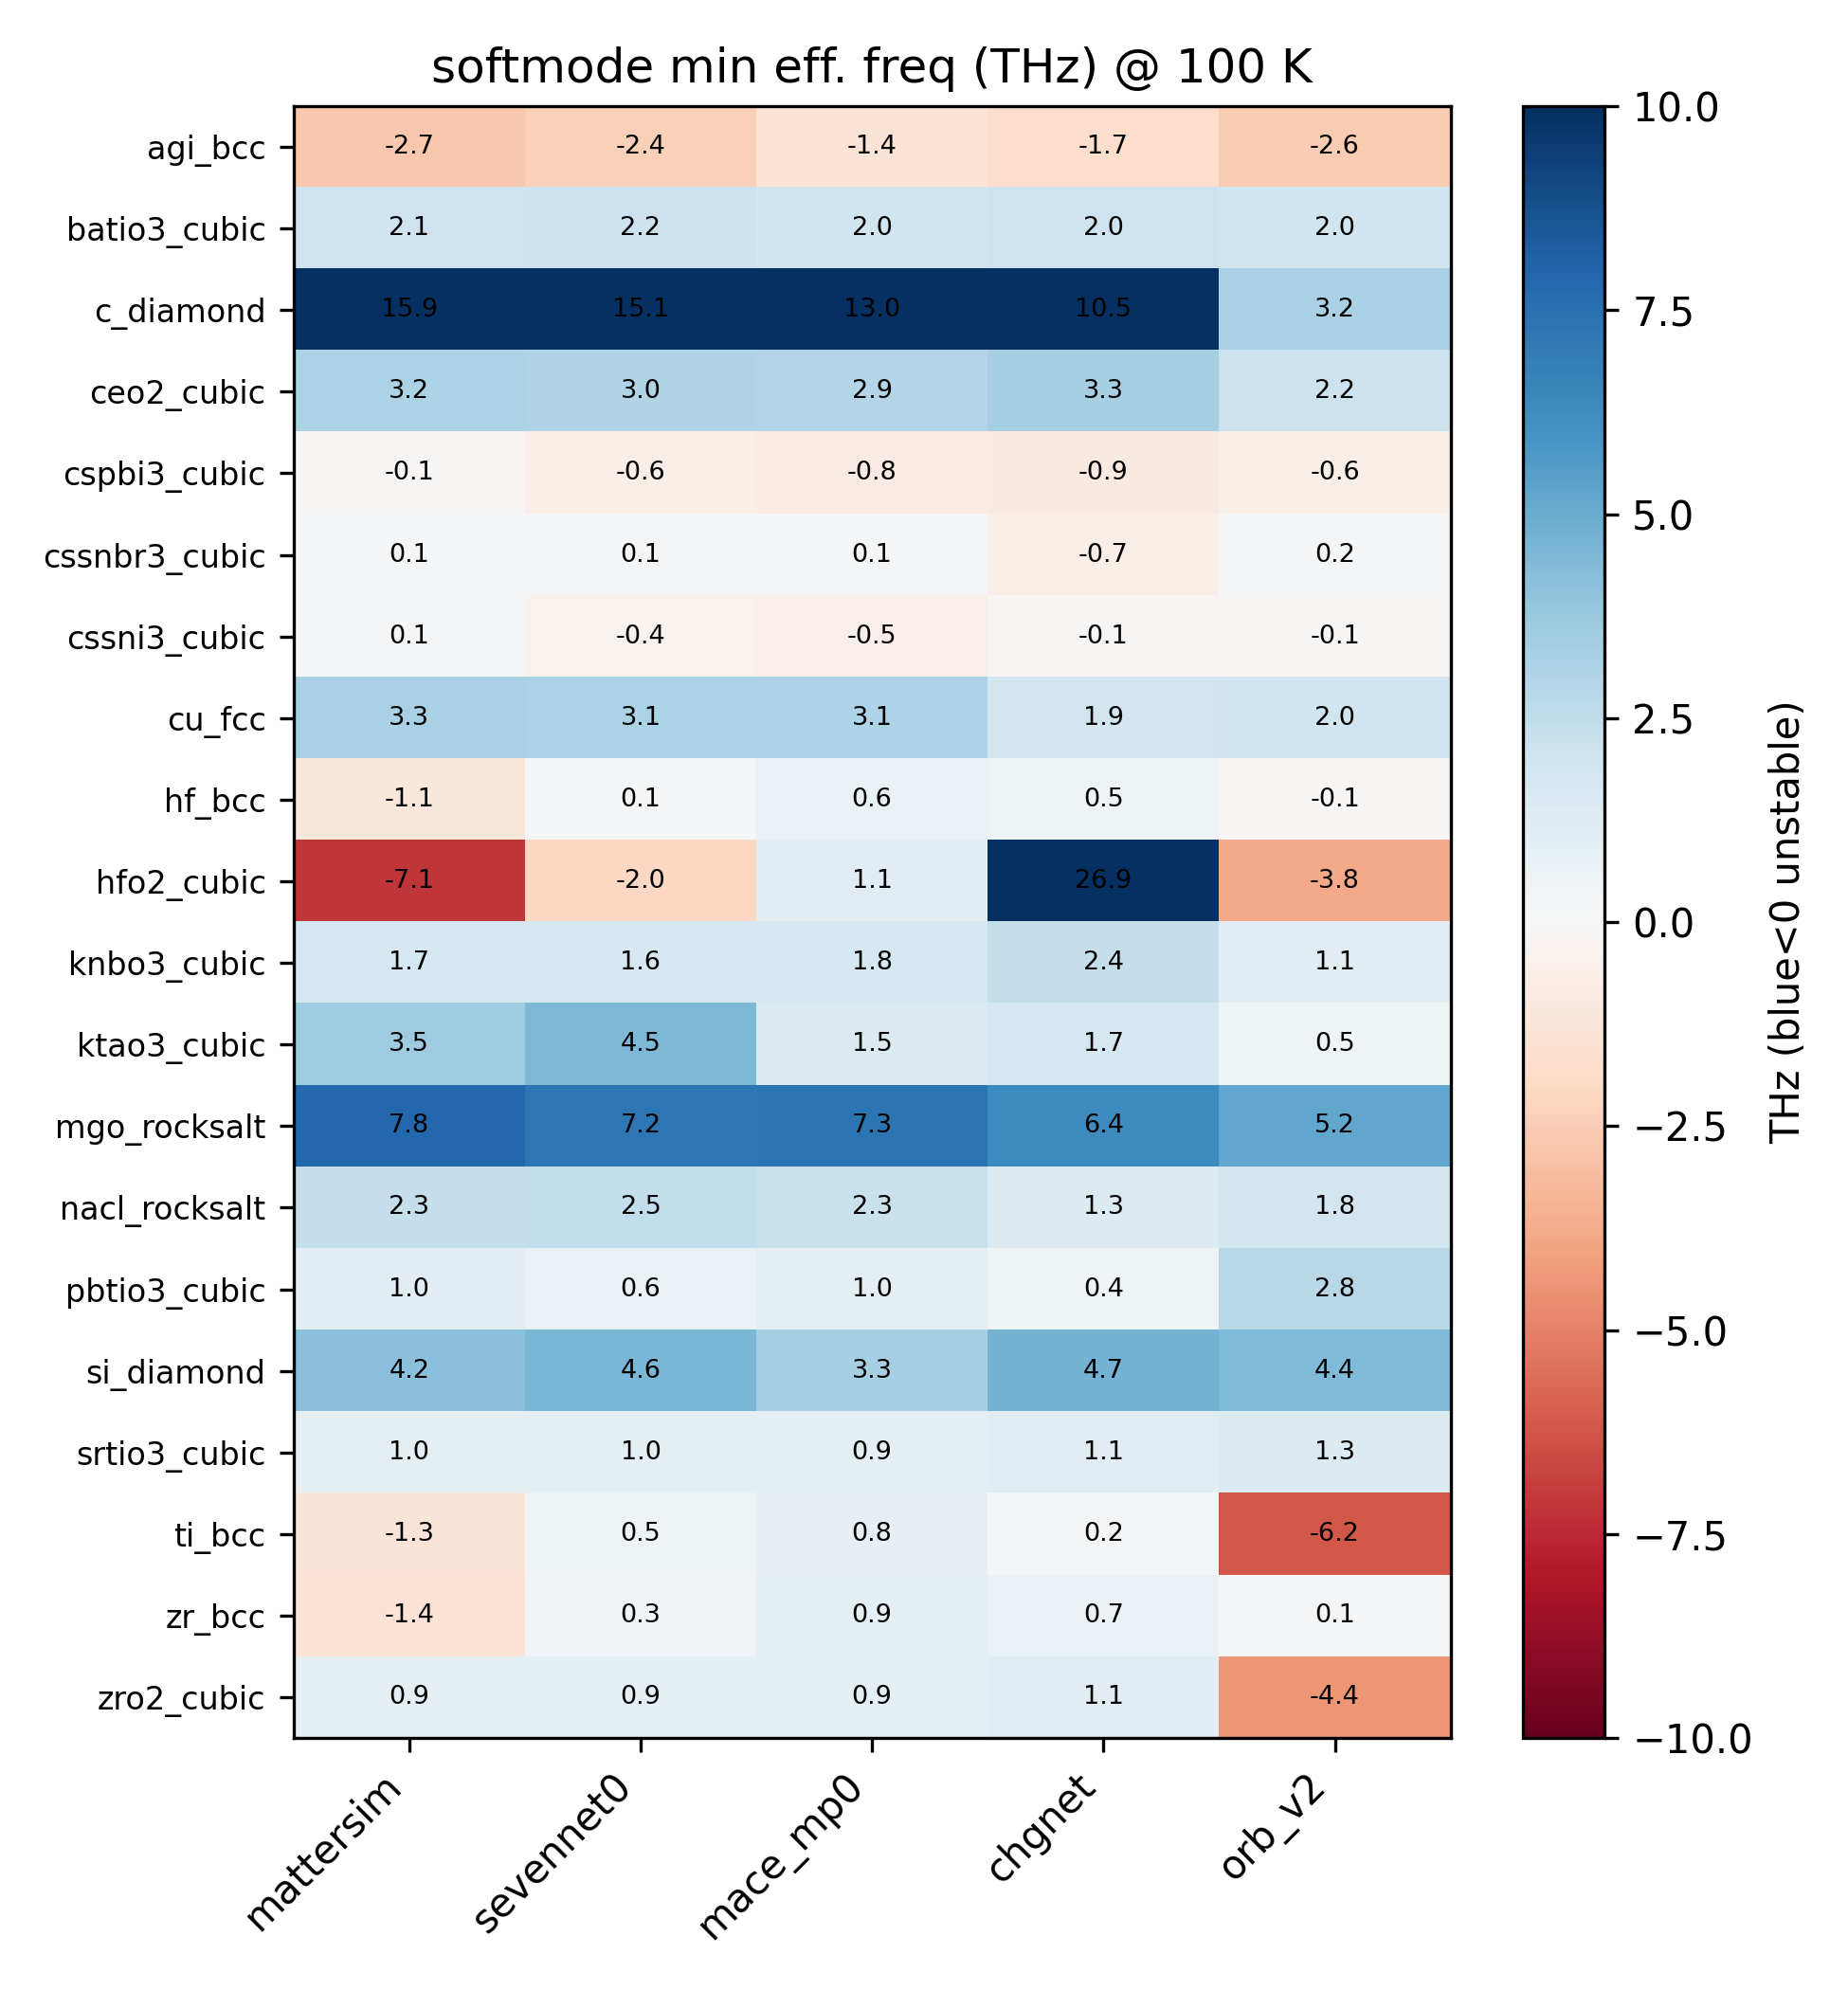
\includegraphics[width=0.85\linewidth]{figures/fig_softmode_heat.png}
\caption{Per-system minimum effective frequency across the five models. The softening toward zero of the harmonically-unstable systems is the physics; per-system minima, not binary rates, are the right reporting unit.}
\label{fig:softmode}
\end{figure}

\subsection{Finite-temperature soft-mode screen: harmonic accuracy does not transfer (H2)}
\label{sec:h2}

On the ferroelectric perovskites at $T\le300$~K, far below every transition temperature, the multi-mode screen correctly calls the cubic phase unstable in 16 of 30 model units (recall 0.53). Across other anharmonic families the screen is stronger: recall 0.92 on halide perovskites, 1.00 on cubic fluorites, 0.60 on the SrTiO$_3$ tilt. On the six harmonically-stable controls it is correct on all 120 model units and finds zero imaginary commensurate modes in every case, so it never manufactures an instability.

\begin{table}[h]
\caption{Finite-temperature false-stable rate and accuracy (non-bcc, non-borderline, $T\le300$~K) against harmonic accuracy.}
\label{tab:finiteT}
\centering
\small
\begin{tabular}{lccc}
\toprule
Model & Finite-T false-stable rate & Finite-T accuracy & (Harmonic accuracy) \\
\midrule
SevenNet-0 & 0.125 & 0.900 & 1.000 \\
CHGNet & 0.188 & 0.867 & 0.789 \\
MatterSim & 0.250 & 0.833 & 1.000 \\
MACE-MP-0 & 0.250 & 0.833 & 0.895 \\
ORB-v2 & 0.312 & 0.800 & 0.895 \\
\bottomrule
\end{tabular}
\end{table}

Read against the harmonic ranking, the ordering is not preserved but neither is it inverted. On the matched non-bcc, non-borderline comparison ($n=75$ system$\times$model pairs) the relationship is temperature-dependent: at 100~K harmonic and finite-temperature correctness are weakly and non-significantly concordant ($\phi=0.149$, McNemar exact $p=0.73$); at 300~K the relationship reverses and becomes significant ($\phi=-0.129$, $p=0.007$), driven by 17 harmonically-correct units mis-called at finite temperature against only 4 the other way. The clearest single demonstration is CHGNet: the \emph{worst} model harmonically (0.789) yet the \emph{second-best} at finite temperature (0.867), while MatterSim is harmonically perfect (1.000) yet only mid-table at finite temperature (0.833). SevenNet-0 leads both layers, so the relationship is not a simple inversion. A top harmonic score therefore does not identify the best finite-temperature screener, and a poor one does not disqualify a model. Full per-family recall, the multi-anchor transition-temperature comparison, and the PbTiO$_3$ ordering failure are reported in Appendix~\ref{app:h2-detail}.

\subsection{SSCHA: clean for bcc, false-stable for perovskites at default truncation}
\label{sec:sscha}

We ran multi-mode SSCHA across both families to cross-validate the screen. The result is asymmetric and is itself a central finding: this concerns SSCHA as realistically deployed with an MLIP force engine for a fixed high-symmetry reference (\texttt{ForcePositiveDefinite} initialisation, 2$\times$2$\times$2 cell, bubble-truncated free-energy Hessian, automatic stochastic relaxation) --- the recipe a practitioner escalating from a cheap screen would run. It is not a claim that the SSCHA formalism is wrong; the formalism anticipates this failure and prescribes its own remedy (Section~\ref{sec:rootcause}), but that remedy is impractical at screening scale.

\textbf{bcc metals: a clean gold standard.} Across Ti/Zr/Hf $\times$ 5 models $\times$ 5 temperatures (75 runs), SSCHA produced zero numerical failures, minimum free-energy-Hessian frequencies in a physical [0.06, 2.1]~THz range, and all five models anharmonically stabilise the bcc phase by $\le\!50$~K (far below the thermodynamic transition, since bcc$\to$hcp/$\omega$ is martensitic and strain-coupled; the thermodynamic $T_c$ is the wrong dynamic-stability comparison). Against the screen, the two methods agree on the stability call in 35 of 45 paired bcc units (sign agreement 0.78; 0.83 excluding ORB-v2), while magnitudes are not rank-correlated (Spearman $\rho=0.11$) --- expected, since a single-mode curvature and a multi-mode Hessian are different observables away from the sign change, so we report call agreement rather than a magnitude correlation.

\textbf{Ferroelectric perovskites: SSCHA systematically false-stabilises.} On the same FE perovskites at $T\le300$~K where the screen reaches 0.53 recall, SSCHA correctly identifies the instability in only 5 of 27 units that return a physical number (recall 0.19); seven units die at symmetry/ensemble assertions, six on PbTiO$_3$ --- the deepest wells in the set. This is the cautionary result: the expensive gold standard is \emph{less} reliable than the cheap screen in the displacive regime that dominates generative-CSP outputs (recall 0.19 against 0.53, with the deepest-well units unable to complete; Figure~\ref{fig:recall}).

\begin{figure}[h]
\centering
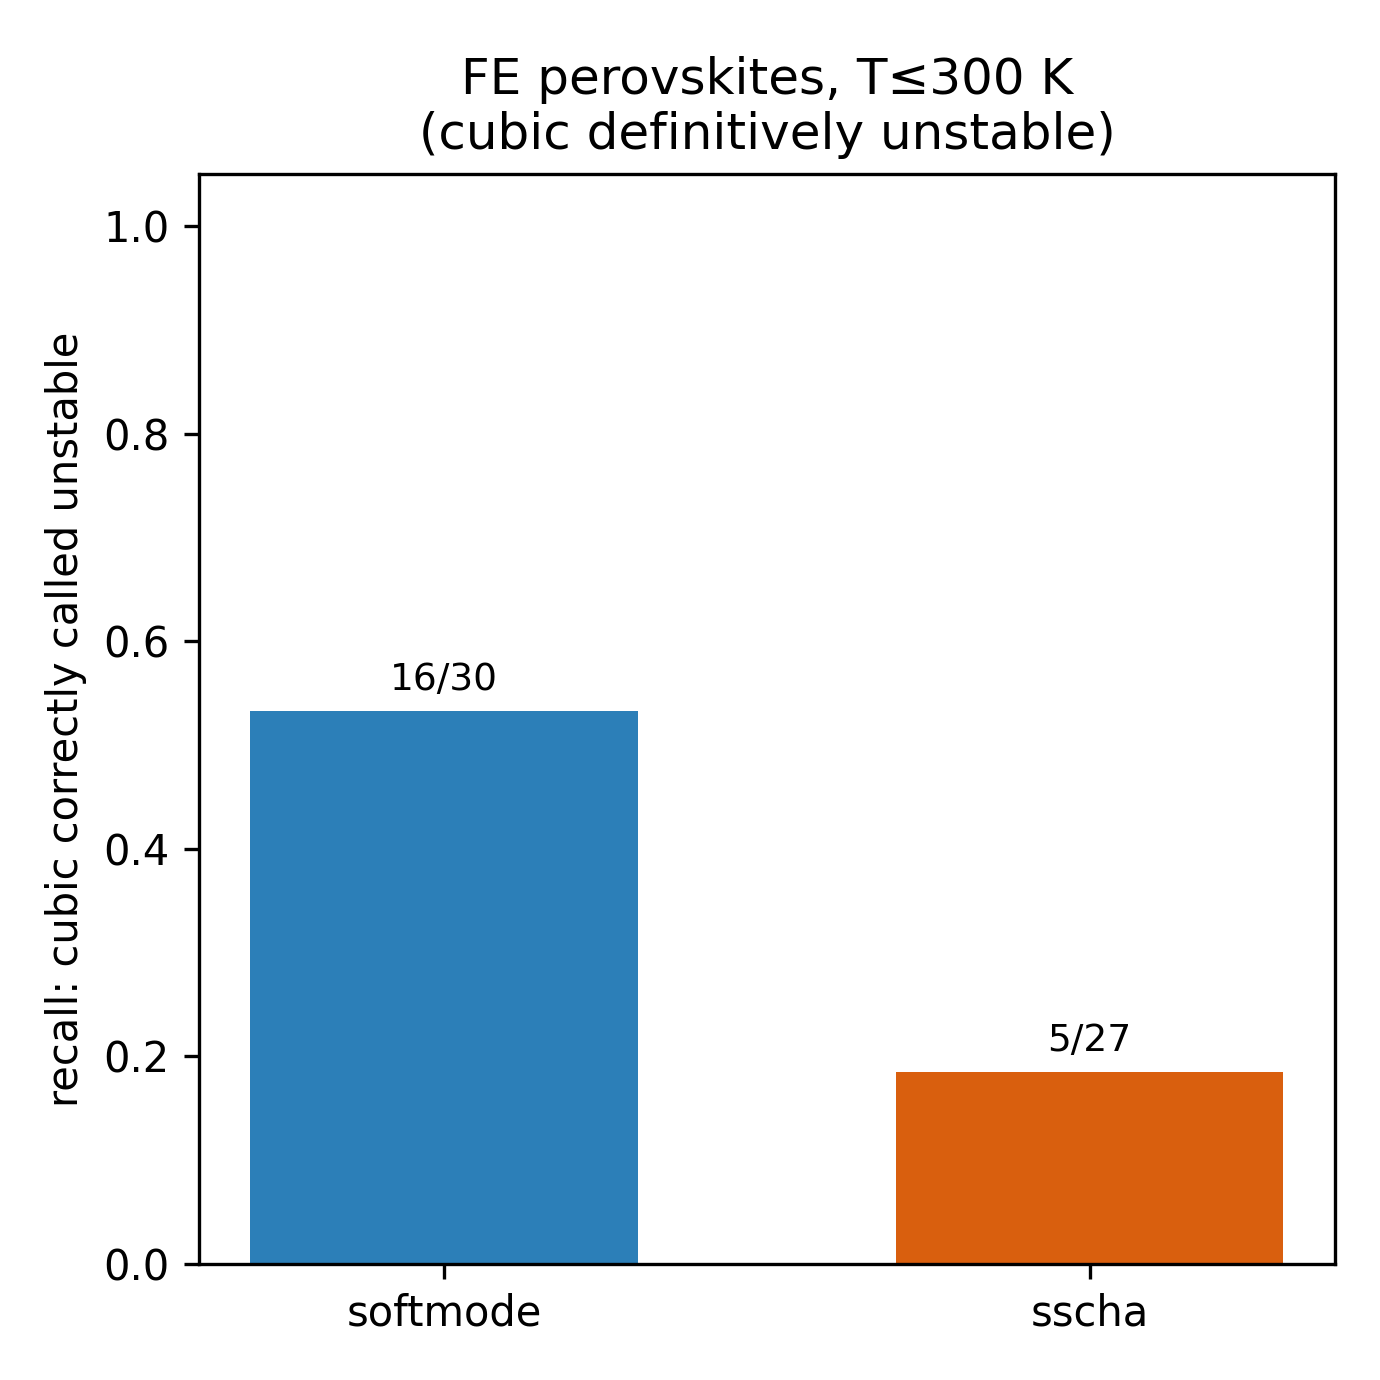
\includegraphics[width=0.7\linewidth]{figures/fig_displacive_recall.png}
\caption{Recall of the displacive (ferroelectric-perovskite) instability at $T\le300$~K: the cheap multi-mode soft-mode screen (0.53) versus the expensive gold-standard SSCHA (0.19).}
\label{fig:recall}
\end{figure}

\subsubsection{Root cause: the fourth-order truncation}
\label{sec:rootcause}

A controlled diagnostic on cubic BaTiO$_3$ isolates the mechanism, and the SCHA literature identifies it precisely. The auxiliary SCHA matrix $\boldsymbol{\Phi}$ is positive-definite by construction, so it can never soften; the object that \emph{can} detect a displacive transition from a fixed high-symmetry reference is the free-energy Hessian $\partial^2F/\partial\mathbf{R}\partial\mathbf{R}=\boldsymbol{\Phi}+\boldsymbol{\Phi}^{(3)}\boldsymbol{\Lambda}[\mathbf{1}-\boldsymbol{\Phi}^{(4)}\boldsymbol{\Lambda}]^{-1}\boldsymbol{\Phi}^{(3)}$ [21]. Our diagnostic shows the failure enters at the truncation: the harmonic soft mode is $-5.6$~THz (correctly unstable), yet with the fourth-order term dropped --- the bubble approximation and the default deployment --- the Hessian returns $+2.87$~THz and the call is false-stable. This is the regime in which the bubble is known to fail; the complete resummation is theoretically required to determine phase stability there [22]. Our contribution is measuring that breakdown at benchmark scale and showing it is not confined to halide perovskites: it holds for oxide perovskites, and, free of stochastic blow-ups, for cubic fluorites too (Appendix~\ref{app:fluorites}), which separates a methodological limit from a numerical one. Enabling the fourth-order term is the physically correct escalation but ran for over 18~minutes on a single unit without finishing and is numerically viable only in float64 --- the practical barrier at screening scale. We therefore use SSCHA as the bcc gold standard and the experimental transition temperature (Section~\ref{sec:screen}) as validation for the perovskite screen.

\subsection{Ensemble disagreement as a guardrail (H3)}
\label{sec:h3}

Because no single model is reliable across the set, we test whether cross-model disagreement flags units where the majority-vote consensus is wrong. On the non-bcc, non-borderline soft-mode units ($n=60$), the consensus is wrong on 20.0\% of units overall. The disagreement signal separates these sharply: on the 14 units where the five models split on the stable/unstable call, the consensus error rate is 0.57, against 0.09 on the 46 unanimous units --- a 6.6$\times$ enrichment. As a ranked predictor of consensus error, the binary vote split reaches AUC 0.76, while the continuous cross-model frequency standard deviation carries no usable signal (AUC 0.36, below chance; Figure~\ref{fig:guardrail}). This refines H3 into a rule with a caveat: the discrete inter-model vote split is a useful, cheap guardrail, but the continuous frequency spread that one might naively threshold is not. Disagreement concentrates near the stability boundary, where split votes coincide with frequencies straddling zero and the call is both most uncertain and most error-prone.

\begin{figure}[h]
\centering
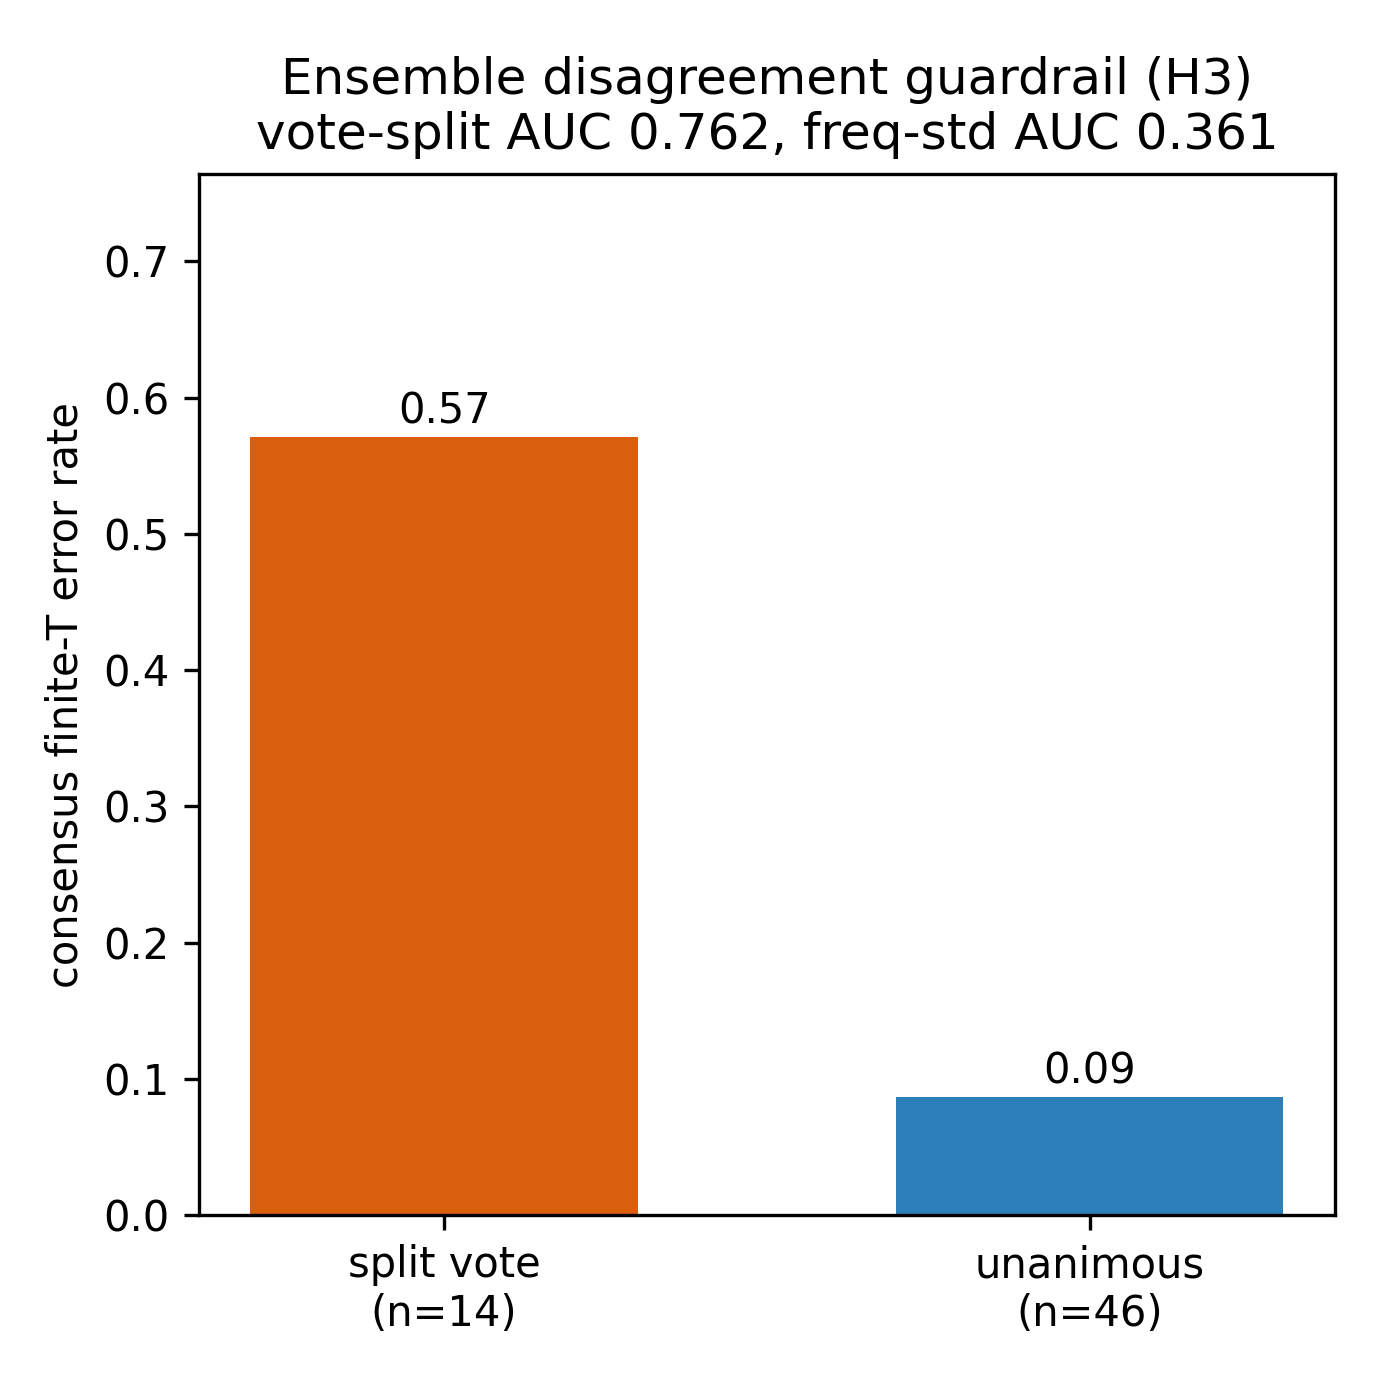
\includegraphics[width=0.7\linewidth]{figures/fig_ensemble_guardrail.png}
\caption{Ensemble-disagreement guardrail: the discrete inter-model vote split predicts consensus error (AUC 0.76) while the continuous cross-model frequency spread does not (AUC 0.36, below chance).}
\label{fig:guardrail}
\end{figure}

Robustness checks --- stochastic-seed reproducibility and finite-size sensitivity, both supporting the headline numbers above --- are reported in Appendix~\ref{app:robustness}.

\section{Discussion}
\label{sec:discussion}

The harmonic layer (Section~\ref{sec:h1}) reproduces the literature and confirms H1: PES softening produces a real false-stable rate, localised to specific instabilities rather than uniform. The finite-temperature results support H2, though with a temperature-dependent statistic rather than a single clean effect: harmonic accuracy is non-predictive of finite-temperature accuracy, and the standard escalation (``if in doubt, run SSCHA'') fails on the displacive regime, because MLIP-driven SSCHA at its default bubble truncation false-stabilises deep double wells. The practical recommendation inverts the usual cost/accuracy intuition: for screening harmonically-unstable displacive candidates, the cheap all-imaginary-mode free-energy screen is the more reliable indicator, and a default-truncation SSCHA escalation should be reserved for martensitic and entropy-stabilised cases, or else run with the fourth-order resummation its own theory prescribes.

\textbf{Limitations.} Ground-truth transition temperatures are approximate and scoring is qualitative. SSCHA cells are 2$\times$2$\times$2 (finite size), so dynamic-stabilisation temperatures are approximate, though the cross-model comparison at fixed cell is valid. ORB-v2's float32-only direct architecture is an outlier in both layers and is flagged throughout rather than excluded. The screen is a single-mode treatment applied mode-by-mode: it captures each instability independently but not their coupling, the most likely reason its predicted stabilisation temperature fails to order PbTiO$_3$ correctly. Both the screen (0.53) and SSCHA (0.19) miss a substantial fraction of the ferroelectric-oxide instabilities, so the comparison identifies the better of two imperfect methods rather than a solved problem.

\section{Conclusions}
\label{sec:conclusions}

Finite-temperature dynamic stability separates foundation MLIPs that the harmonic benchmarks used to certify them rank equally. A cheap quantum free-energy screen, applied to every imaginary commensurate mode rather than to the softest one, recovers finite-temperature behaviour that harmonic accuracy does not predict, and it outperforms MLIP-driven SSCHA at its default bubble truncation on the deep displacive instabilities that dominate generative-CSP screening. Which mode is examined matters as much as which method is used: the deepest instability need not be the one that condenses, and in SrTiO$_3$ it is not. Harmonic accuracy does not certify a model for finite-temperature use, and neither does an unexamined SSCHA cross-check.

\begin{ack}
\end{ack}

\section*{References}

\small
\begin{enumerate}[leftmargin=*,itemsep=0pt,topsep=2pt,label={[\arabic*]}]
\item A. Loew, D. Sun, H.-C. Wang, S. Botti and M. A. L. Marques, \textit{npj Comput. Mater.}, 2025, \textbf{11}, 178.
\item X.-Q. Han, P.-J. Guo, Z.-F. Gao, W.-K. Li and Z.-Y. Lu, \textit{arXiv}, 2025, arXiv:2512.21227.
\item G. Petretto, S. Dwaraknath, H. P. C. Miranda, D. Winston, M. Giantomassi, M. J. van Setten, X. Gonze, K. A. Persson, G. Hautier and G.-M. Rignanese, \textit{Sci. Data}, 2018, \textbf{5}, 180065.
\item L. Monacelli, R. Bianco, M. Cherubini, M. Calandra, I. Errea and F. Mauri, \textit{J. Phys.: Condens. Matter}, 2021, \textbf{33}, 363001.
\item O. Hellman, I. A. Abrikosov and S. I. Simak, \textit{Phys. Rev. B}, 2011, \textbf{84}, 180301(R); O. Hellman, P. Steneteg, I. A. Abrikosov and S. I. Simak, \textit{Phys. Rev. B}, 2013, \textbf{87}, 104111.
\item I. Batatia, P. Benner, Y. Chiang, A. M. Elena, D. P. Kov\'{a}cs, J. Riebesell \textit{et al.}, \textit{arXiv}, 2023, arXiv:2401.00096.
\item B. Deng, P. Zhong, K. Jun \textit{et al.}, \textit{Nat. Mach. Intell.}, 2023, \textbf{5}, 1031.
\item M. Neumann, J. Gin, B. Rhodes, S. Bennett, Z. Li, H. Choubisa, A. Hussey and J. Godwin, \textit{arXiv}, 2024, arXiv:2410.22570.
\item Y. Park, J. Kim, S. Hwang and S. Han, \textit{J. Chem. Theory Comput.}, 2024, \textbf{20}, 4857.
\item H. Yang, C. Hu, Y. Zhou \textit{et al.}, \textit{arXiv}, 2024, arXiv:2405.04967.
\item T. Tadano and S. Tsuneyuki, \textit{Phys. Rev. B}, 2015, \textbf{92}, 054301.
\item W. Zhong, D. Vanderbilt and K. M. Rabe, \textit{Phys. Rev. Lett.}, 1994, \textbf{73}, 1861.
\item A. Marronnier \textit{et al.}, \textit{ACS Nano}, 2018, \textbf{12}, 3477.
\item L. Monacelli and N. Marzari, \textit{Chem. Mater.}, 2023, DOI: 10.1021/acs.chemmater.2c03475.
\item W. Petry \textit{et al.}, \textit{Phys. Rev. B}, 1991, \textbf{43}, 10933; A. Heiming \textit{et al.}, \textit{Phys. Rev. B}, 1991, \textbf{43}, 10948.
\item K. Parlinski, Z. Q. Li and Y. Kawazoe, \textit{Phys. Rev. Lett.}, 1997, \textbf{78}, 4063.
\item D. A. Wood and N. Marzari, \textit{Phys. Rev. B}, 2007, \textbf{76}, 134301.
\item A. Ranalli \textit{et al.}, \textit{Adv. Quantum Technol.}, 2023, \textbf{6}, 2200131.
\item J. Yang, Z. Yin, L. Ao and S. Li, \textit{Phys. Chem. Chem. Phys.}, 2026, \textbf{28}, 4459--4469.
\item \textit{Are Foundational Atomistic Models Reliable for Finite-Temperature Molecular Dynamics?}, \textit{J. Phys. Chem. C}, 2025, DOI: 10.1021/acs.jpcc.5c07541.
\item R. Bianco, I. Errea, L. Paulatto, M. Calandra and F. Mauri, \textit{Phys. Rev. B}, 2017, \textbf{96}, 014111.
\item L. Monacelli, \textit{Phys. Rev. B}, 2025, \textbf{112}, 014109.
\item D. J. Hooton, \textit{Philos. Mag.}, 1955, \textbf{46}, 422.
\item N. R. Werthamer, \textit{Phys. Rev. B}, 1970, \textbf{1}, 572.
\item R. Peierls, \textit{Phys. Rev.}, 1938, \textbf{54}, 918.
\item R. P. Feynman, \textit{Statistical Mechanics: A Set of Lectures}, W. A. Benjamin, Reading, MA, 1972.
\end{enumerate}
\normalsize

%%%%%%%%%%%%%%%%%%%%%%%%%%%%%%%%%%%%%%%%%%%%%%%%%%%%%%%%%%%%
\appendix

\section{Data and code availability}
\label{app:data}
Code and the per-unit results ledger will be released at a persistent archive upon acceptance; withheld here for double-blind review. The production results regenerate deterministically from an append-only, per-unit-hashed ledger (unit hashes include the method version, so a re-run under a changed algorithm records new rows rather than silently reusing old ones); every figure and statistic in this paper is computed through that ledger. Each model was run in its own pinned virtual environment.

\section{Full variational derivation of the soft-mode screen}
\label{app:derivation}
The trial density in Section~\ref{sec:screen} is a Gaussian of mean $Q_0$ and quantum width
\[
\sigma^2=\frac{\hbar}{2M\Omega}\coth\!\left(\frac{\hbar\Omega}{2k_BT}\right),
\]
which carries the nuclear quantum effects: at high $T$ it recovers the classical $k_BT/M\Omega^2$, and at $T\to0$ it retains the zero-point width that suppresses condensation in shallow wells (quantum paraelectricity). The Gaussian expectation of the even sextic follows from the moments $\langle Q^2\rangle=Q_0^2+\sigma^2$, $\langle Q^4\rangle=Q_0^4+6Q_0^2\sigma^2+3\sigma^4$, $\langle Q^6\rangle=Q_0^6+15Q_0^4\sigma^2+45Q_0^2\sigma^4+15\sigma^6$. Stationarity of $\mathcal{F}$ with respect to $\Omega$ at fixed $Q_0$ gives the self-consistency condition
\[
M\Omega^2=\langle V''\rangle_{Q_0,\sigma}=2a+12b\langle Q^2\rangle+30c\langle Q^4\rangle,
\]
solved by bracketed root finding on $\sigma^2$ (avoiding the runaway large-$\sigma$ fixed point a damped iteration can reach); $\mathcal{F}$ is then minimised over the centroid on a $Q_0$ grid. The $E(Q)$ maps are temperature-independent and cached, so each temperature is a sub-second CPU solve over all modes. A cap of 24 modes per unit bounds cost; it binds on 20 of 400 units, every one of which is already called unstable with at least three condensing modes, so it cannot affect any call. Three earlier finite-temperature routes (hand-rolled TDEP [5], one-shot hiPhive, rattled-MD) were implemented and discarded after failing the SrTiO$_3$ gate.

\section{Screen approximation ledger}
\label{app:approx}
\begin{table}[h]
\centering
\scriptsize
\begin{tabular}{L{0.045\linewidth}L{0.185\linewidth}L{0.255\linewidth}L{0.16\linewidth}L{0.22\linewidth}}
\toprule
\# & Approximation & What it excludes & Expected bias & Where it shows \\
\midrule
A1 & One mode at a time & Mode coupling, cooperative condensation & Either sign; $T^*$ unreliable & PbTiO$_3$ $T^*$ ordering fails (App.~\ref{app:h2-detail}) \\
A2 & Commensurate $\mathbf{q}$ only & Incommensurate/finer-grid instabilities & False-stable if true mode missed & R point needs even cells; bcc needs 6$\times$6$\times$6 FCs \\
A3 & Sextic fit, well+barrier window & Steep-wall anharmonicity beyond $Q^6$ & Barrier-shape error at large $Q$ & Fit-window sensitivity study \\
A4 & Gaussian trial state & Tunnelling, non-Gaussian density & Curvature misses condensation & Blind rows; Sec.~\ref{sec:rootcause} \\
A5 & Static $E(Q)$, clamped cell & Thermal expansion, strain coupling & Under-stabilises martensitic systems & bcc labelled via SSCHA instead \\
A6 & Mode cap (24) & Modes beyond 24 most imaginary & Could only create false-stables & Binds on 20/400, all already unstable \\
\bottomrule
\end{tabular}
\caption{The screen's approximation ledger, declared.}
\end{table}

\section{Finite-temperature screen: additional detail (H2)}
\label{app:h2-detail}
Beyond the SrTiO$_3$ gate we compare the screen's predicted stabilisation temperature $T^*$ (lowest ladder $T$ at which the phase is called stable) against experimental transition temperatures. SrTiO$_3$ ($T_c\approx105$~K) stabilises earliest, at $T^*=100$--300~K, and BaTiO$_3$ (393~K) and KNbO$_3$ (708~K) follow at $T^*=300$~K for four of five models, so the SrTiO$_3$-below-ferroelectric ordering holds. PbTiO$_3$ (763~K), the highest transition temperature of the four, does \emph{not} follow: $T^*$ is 100~K for three models, 600~K and 900~K for the other two. This is a genuine ordering failure rather than a scale error and is the clearest limitation of the screen; $T^*$ is reported as a diagnostic, not as what licenses the screen (the SrTiO$_3$ gate and control performance do that).

\section{SSCHA root-cause and fluorite confirmation}
\label{app:fluorites}
Cubic ZrO$_2$ (the $>$2600~K phase, harmonically unstable via the X-point oxygen mode at all temperatures studied) is a cleaner test than the perovskites because its instability is shallower and does not trigger float32 blow-ups. The soft-mode screen calls both fluorites unstable at every temperature and for every model (recall 1.00). SSCHA instead returns $+2.0$ to $+3.3$~THz at 100~K for all five models on ZrO$_2$ (false-stable), and for HfO$_2$ shows the same pattern ($+1.9$ to $+2.6$~THz at 100~K). Across both fluorites SSCHA produced zero numerical blow-ups yet the same systematic false-stable behaviour, confirming the failure is methodological rather than numerical.

\section{Robustness: stochastic noise and finite size}
\label{app:robustness}
\textbf{Stochastic reproducibility.} Repeating one bcc-Zr/MACE-MP-0/100~K SSCHA unit with four independent random seeds gives a minimum free-energy-Hessian frequency of $+1.798\pm0.001$~THz, two-to-three orders of magnitude smaller than the cross-model bcc margins reported in Section~\ref{sec:sscha}, so those margins are real signal rather than sampling noise.

\textbf{Finite size.} The SSCHA stability call is insensitive to supercell size where the test is well-posed: for bcc-Zr the dynamic-stabilisation verdict holds from 2$\times$2$\times$2 to 3$\times$3$\times$3. One caveat is intrinsic to the physics: the SrTiO$_3$ antiferrodistortive instability lives at the zone-boundary R point, commensurate only with even supercells, so a 3$\times$3$\times$3 cell is blind to it by construction; a definitive even-cell test (4$\times$4$\times$4) is left to future work. The Section~\ref{sec:sscha} SSCHA false-stable is not a missing-$\mathbf{q}$ artifact: it occurs for the $\Gamma$ ferroelectric mode of BaTiO$_3$, present in every cell including the 2$\times$2$\times$2 used, so the failure is the fourth-order truncation identified in Section~\ref{sec:rootcause}, not finite size.

\textbf{Harmonic tolerance sweep.} A strict tolerance (0~THz) floods false-unstables (29 calls) as near-$\Gamma$ finite-displacement noise dominates, while a loose tolerance (0.3~THz) inflates false-stables (7 calls); the default $-0.1$~THz sits in the stable basin between them (5 false-stable, 3 false-unstable), and the split holds across 0.05--0.2~THz.

\newpage
\section*{SIMBIOCHEM Submission Checklist}

%%% BEGIN INSTRUCTIONS %%%
For SIMBIOCHEM II this checklist is \textbf{highly encouraged but not enforced}. Omitting it, or answering \answerNo{}/\answerNA{}, is \emph{not} grounds for desk rejection. Its purpose is to encourage responsible research and transparency --- in particular the \textbf{disclosure of AI/LLM use} and adherence to \textbf{research-integrity} norms. The checklist does not count towards the page limit and should follow the references and any appendices.

For each item you choose to answer, use \answerYes{}, \answerNo{}, or \answerNA{}, followed by a short (1--2 sentence) justification. You may delete this instruction block but please keep the section heading.
%%% END INSTRUCTIONS %%%


\begin{enumerate}

\item {\bf Claims}
    \item[] Question: Do the main claims in the abstract and introduction accurately reflect the paper's contributions and scope?
    \item[] Answer: \answerYes{}
    \item[] Justification: The abstract and introduction state exactly the three pre-registered findings reported in Section~3 (the harmonic-level model divide, the finite-temperature accuracy gap, and the SSCHA default-truncation false-stabilisation) and the ensemble guardrail result, with no broader claim made.

\item {\bf Limitations}
    \item[] Question: Does the paper discuss the limitations of the work?
    \item[] Answer: \answerYes{}
    \item[] Justification: Section~4 states the approximate/qualitative ground-truth labels, the 2$\times$2$\times$2 SSCHA cell size, the ORB-v2 float32 outlier status, and the single-mode screen's inability to capture mode--mode coupling; Appendix~C tabulates every declared approximation with its expected bias.

\item {\bf AI / LLM disclosure} \emph{(important)}
    \item[] Question: Does the paper disclose any use of AI/LLMs in the research or writing (e.g., ideation, code generation, data processing, drafting), in line with the NeurIPS LLM policy?
    \item[] Answer: \answerYes{}
    \item[] Justification: An AI coding/writing assistant (Claude) was used throughout the underlying research repository, under the author's direction, to implement the benchmark harness and analysis code and to draft and audit manuscript text, and was used to condense this workshop submission from the full-length manuscript under review elsewhere. The author reviewed, verified against the results ledger, and takes full responsibility for all reported results and text.
    \item[] Guidelines:
    \begin{itemize}
        \item Briefly describe the scope of any AI/LLM assistance. The authors remain fully responsible for the correctness, originality, and integrity of all content.
    \end{itemize}

\item {\bf Research integrity \& originality}
    \item[] Question: Do you confirm that this is an original submission --- not a duplicate or lightly tweaked resubmission, nor one of multiple versions of the same work submitted to this workshop --- and that you comply with research-integrity guidelines?
    \item[] Answer: \answerYes{}
    \item[] Justification: This is the only submission of this work to this workshop. A full-length version is concurrently under review at a journal, which the SIMBIOCHEM CFP explicitly permits (``currently under review elsewhere''); no tweaked duplicate has been or will be submitted here.
    \item[] Guidelines:
    \begin{itemize}
        \item SIMBIOCHEM runs mechanisms to detect the same paper being submitted multiple times with tweaks. Such attempts are reported to OpenReview and NeurIPS as misconduct and are desk-rejected.
    \end{itemize}

\item {\bf Reproducibility} \emph{(optional)}
    \item[] Question: Where applicable, does the paper provide enough information (data, code, settings) to reproduce the main results?
    \item[] Answer: \answerYes{}
    \item[] Justification: All results derive from an append-only, per-unit-hashed ledger regenerable from the pinned per-model environments and cached intermediate free-energy maps described in Appendix~A; code and data will be released at a persistent archive upon acceptance (withheld pre-acceptance for double-blind review).

\end{enumerate}


\end{document}
